\documentclass[12pt,halfline,a4paper]{ouparticle}
\usepackage{tabularx}
\usepackage{graphicx}

\begin{document}

\title{Sample Article for\break {Oxford University Press~Journals}}

\author{%
\name{Lucas Reeh}
\email{lreeh@student.tugraz.at}
}
\date{\today}

\keywords{computational intelligence, assignement1}

\begin{titlepage}
   \begin{center}
     \begin{huge}
		   %% Update assignment number here
           \textbf{Assignment 1}
     \end{huge}
   \end{center}

   \begin{center}
     \begin{large}
           Computational Intelligence, SS2017
     \end{large}
   \end{center}

   \begin{center}
 \begin{tabularx}{\textwidth}{|>{\hsize=.33\hsize}X|>{\hsize=.33\hsize}X|>{\hsize=.33\hsize}X|} 

           \hline
           \multicolumn{3}{|c|}{\textbf{Team Members}} \\
           \hline
           Last name & First name & Matriculation Number \\
           \hline
           Reeh & Lucas & 00630128 \\
           \hline

     \end{tabularx}
   \end{center}
\end{titlepage}

\tableofcontents
\listoffigures

\newpage

\section{Linear Regression}

\subsection{Derivation of Regularized Linear Regression}

\subsection{Linear Regression with polynomial features}
	\begin{figure}[H]
	\centering
	        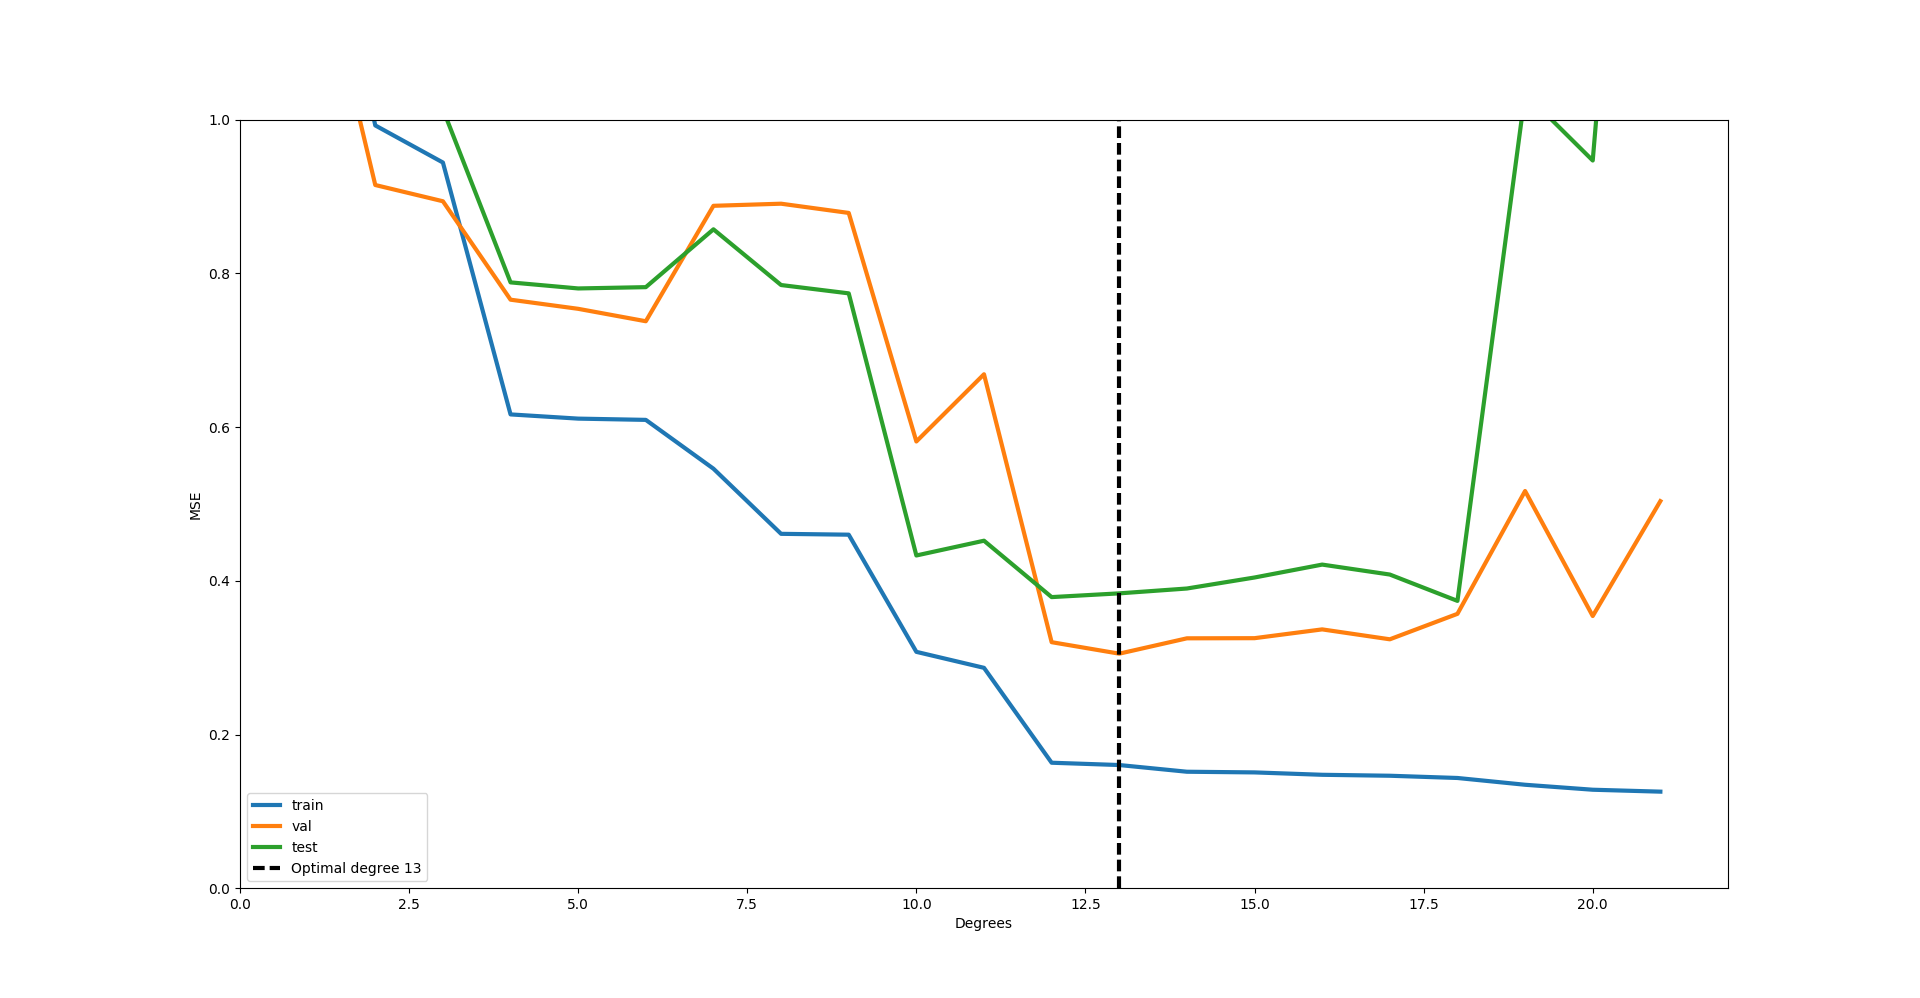
\includegraphics[width=\textwidth]{figures/linreg_errors.png}
	    \caption{Training, validation and testing errors}
	\end{figure}
	\begin{figure}[H]
	\centering
	        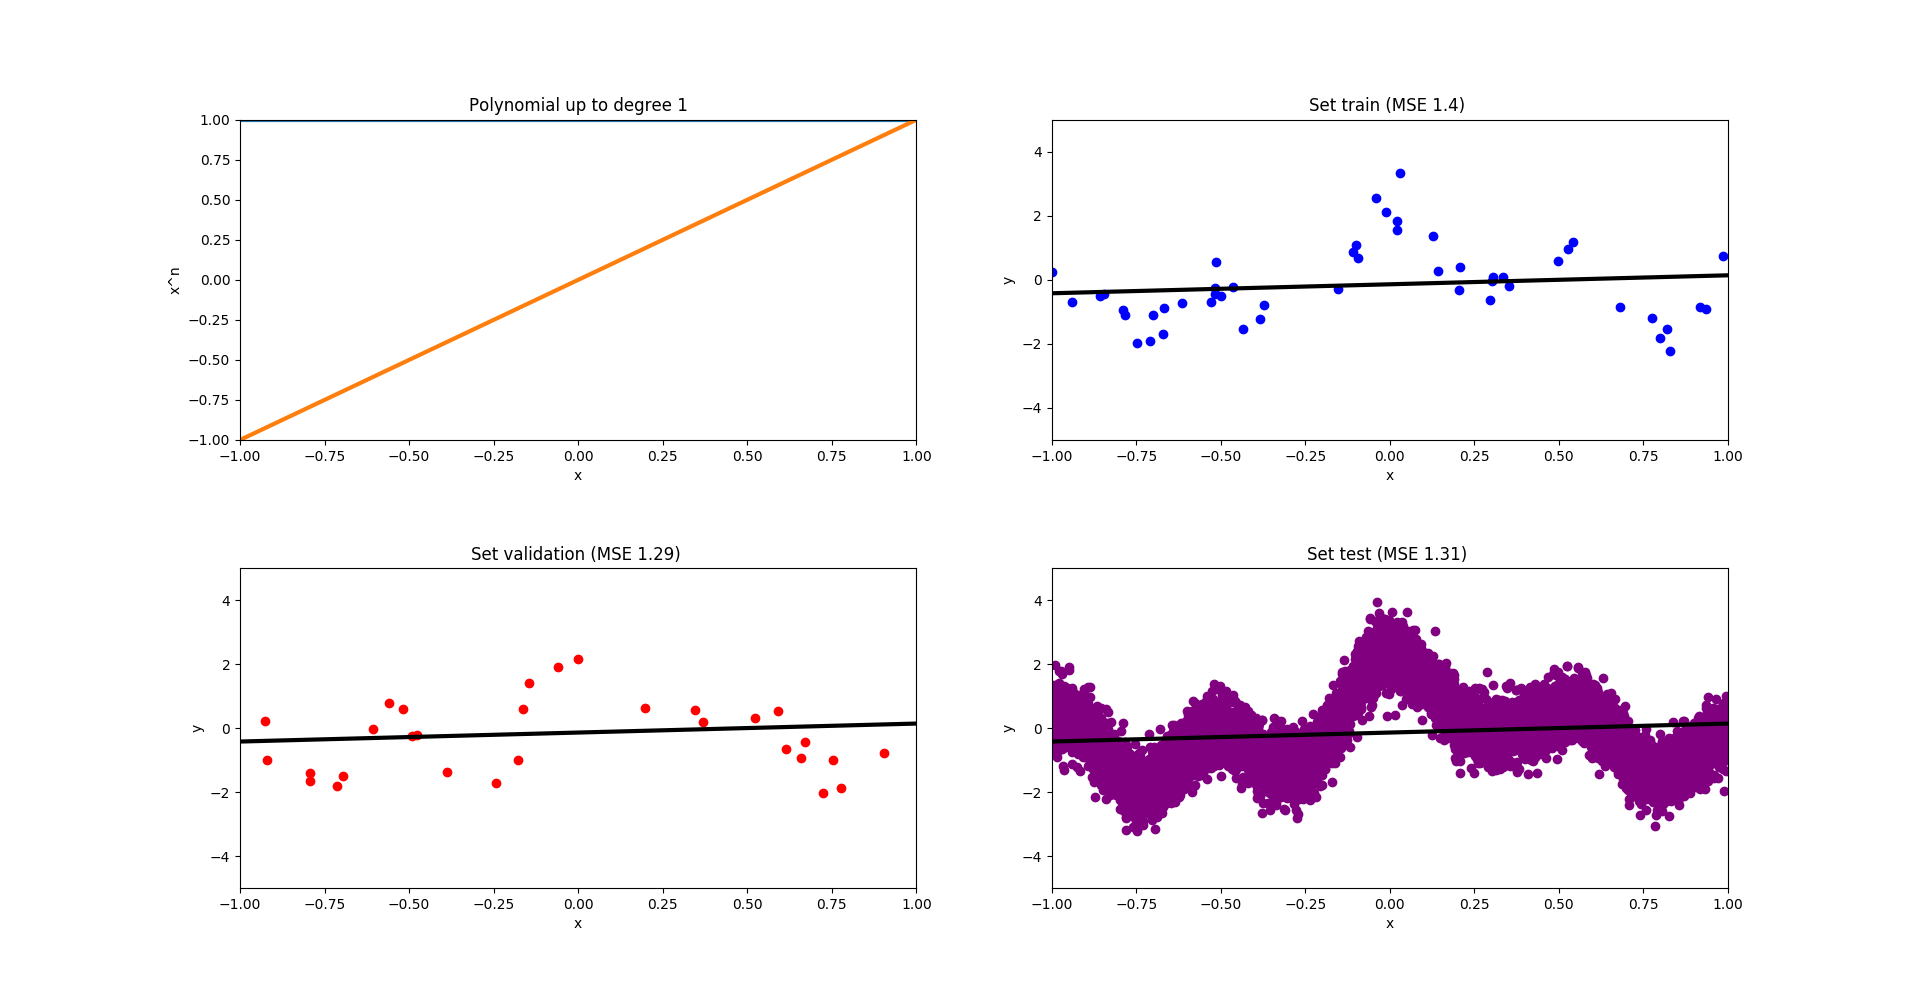
\includegraphics[width=\textwidth]{figures/linreg_degree_1.png}
	    \caption{Linear Regression (Polynomial, Degree 1)}
	\end{figure}
	\begin{figure}[H]
	\centering
	        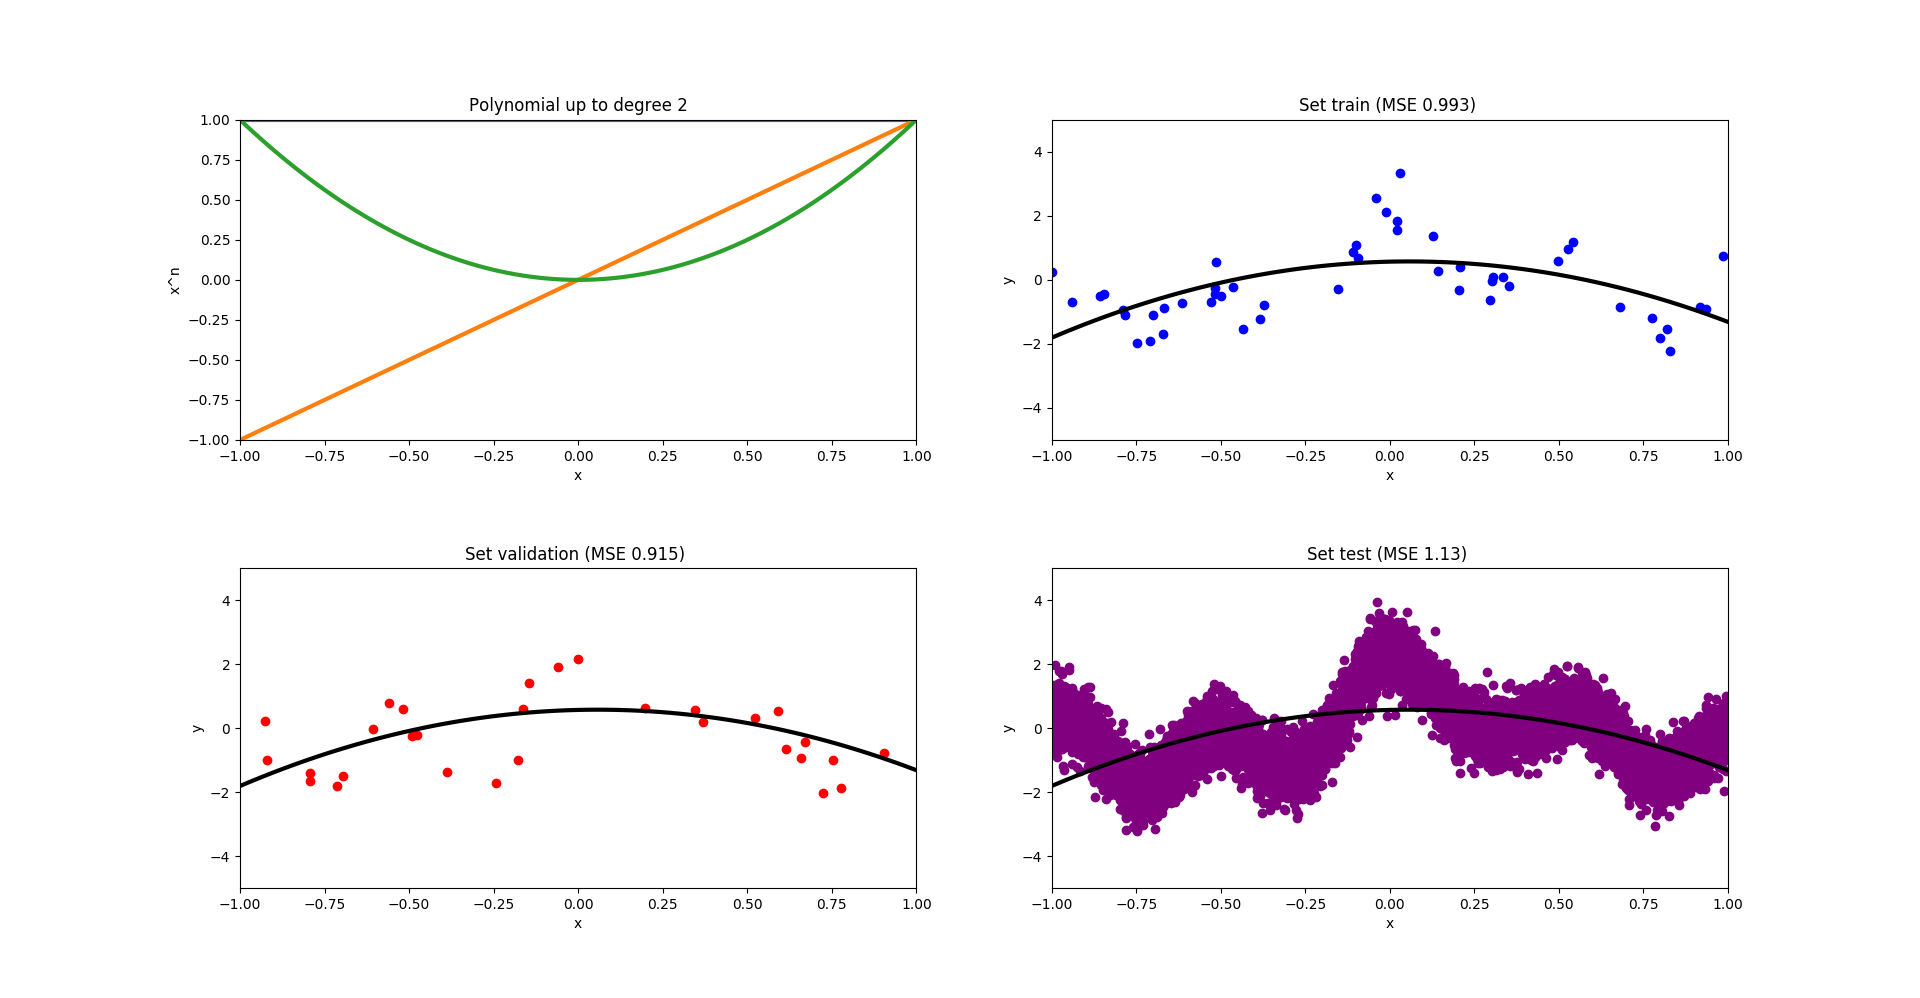
\includegraphics[width=\textwidth]{figures/linreg_degree_2.png}
	    \caption{Linear Regression (Polynomial, Degree 2)}
	\end{figure}
	\begin{figure}[H]
	\centering
	        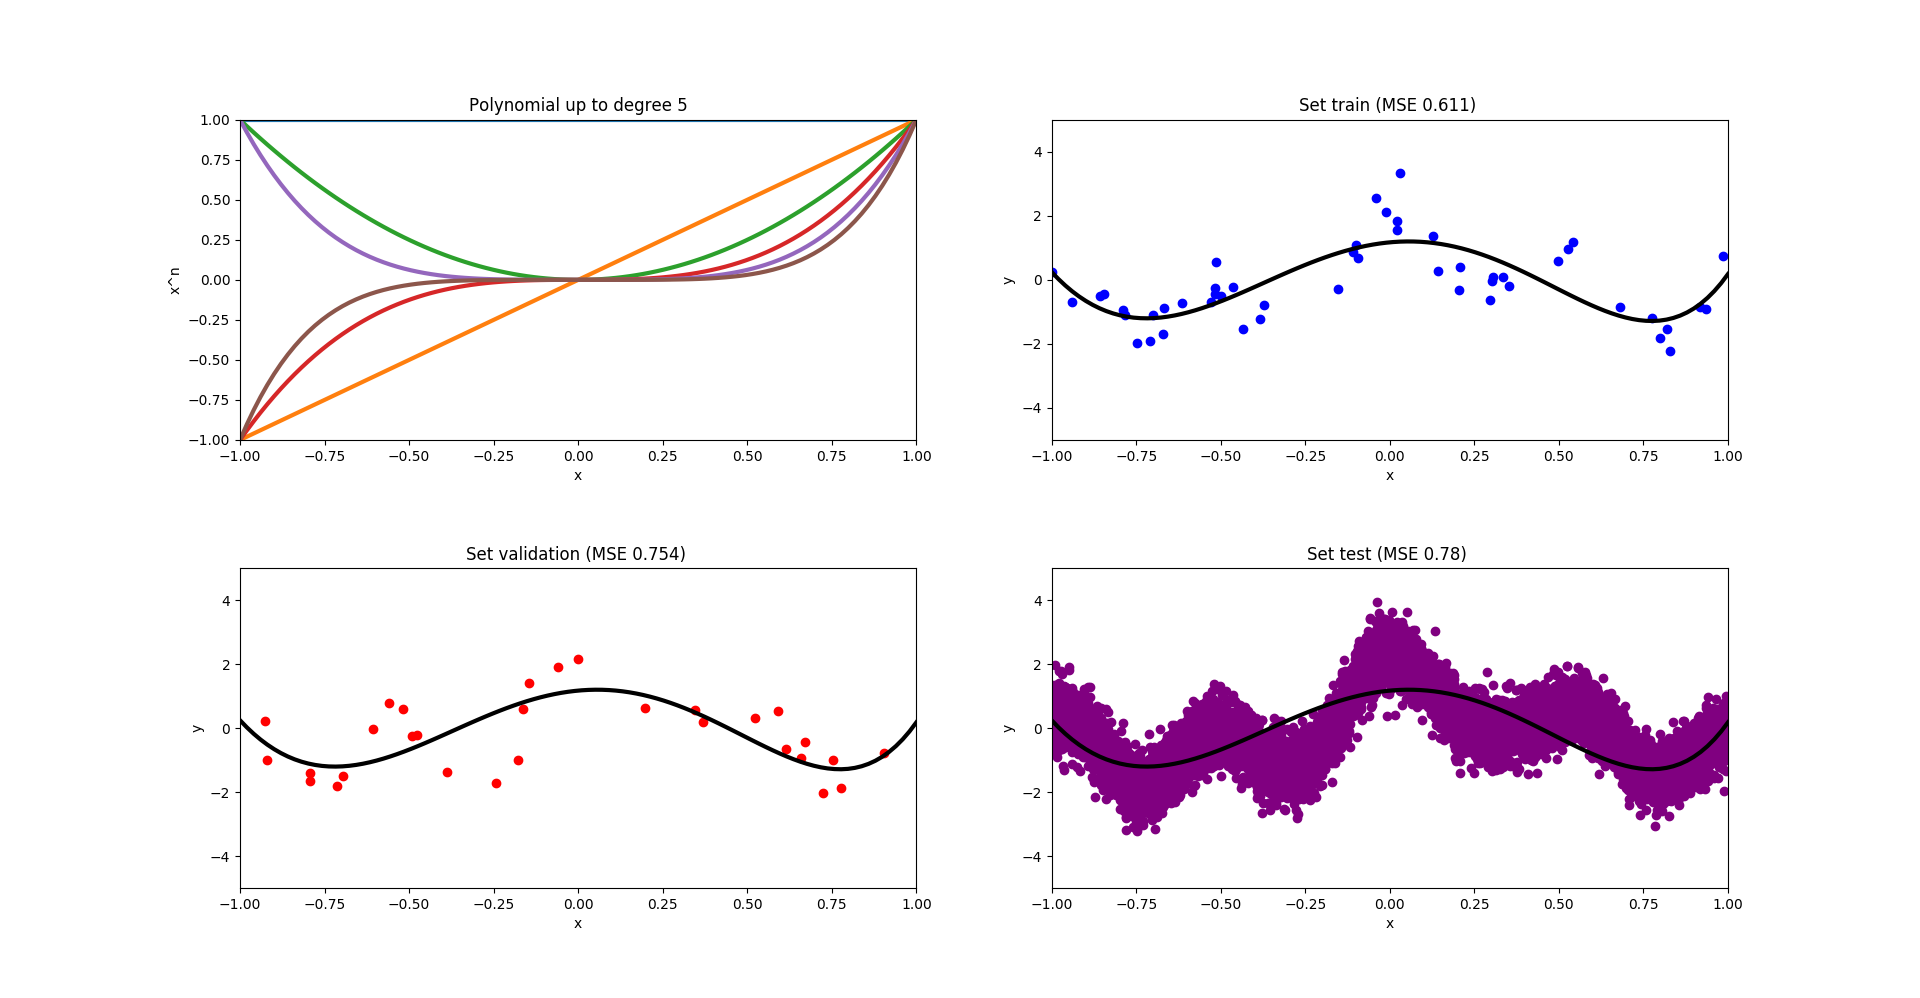
\includegraphics[width=\textwidth]{figures/linreg_degree_5.png}
	    \caption{Linear Regression (Polynomial, Degree 5)}
	\end{figure}
	\begin{figure}[H]
	\centering
	        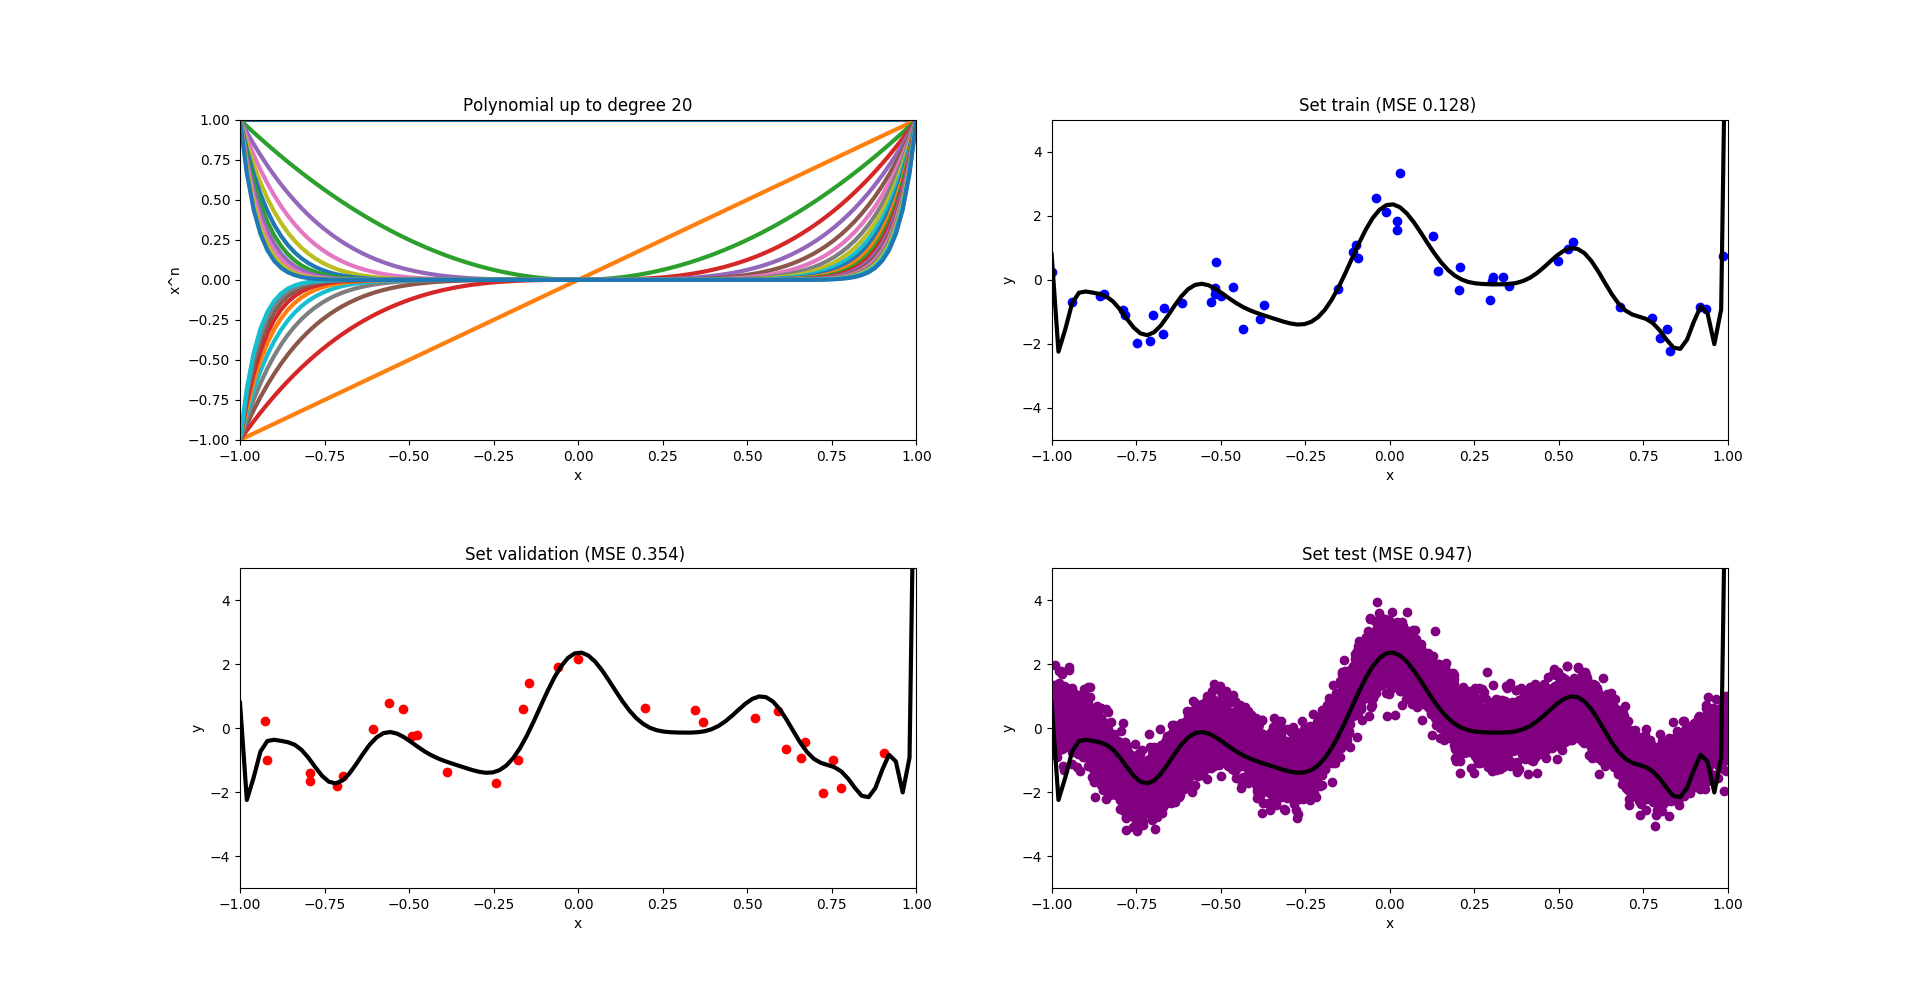
\includegraphics[width=\textwidth]{figures/linreg_degree_20.png}
	    \caption{Linear Regression (Polynomial, Degree 20)}
	\end{figure}
		
\begin{itemize}
  \item Lowest training error when using degree 21
  	\begin{figure}[H]
    \centering
	        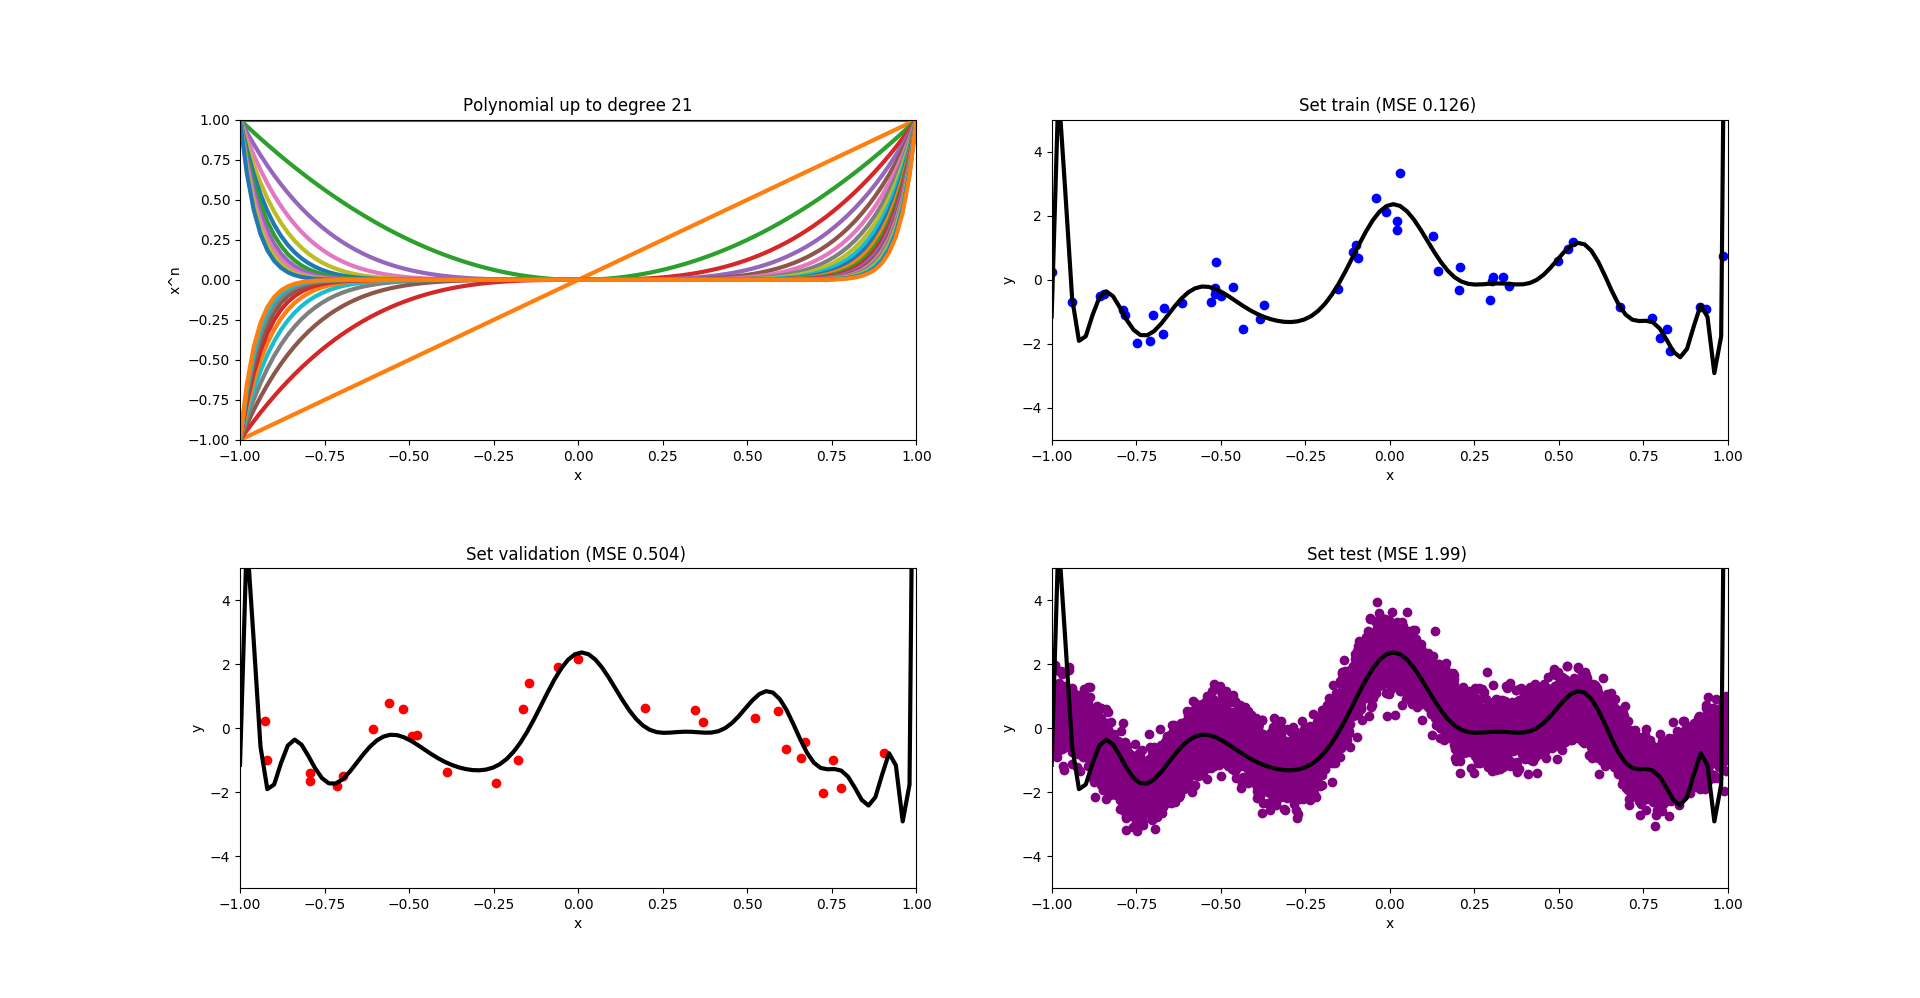
\includegraphics[width=\textwidth]{figures/linreg_degree_21.png}
	    \caption{Linear Regression (Polynomial, Degree 21)}
	\end{figure}
  \item Lowest validation error occurs when using degree 13
	\begin{figure}[H]
    \centering
	        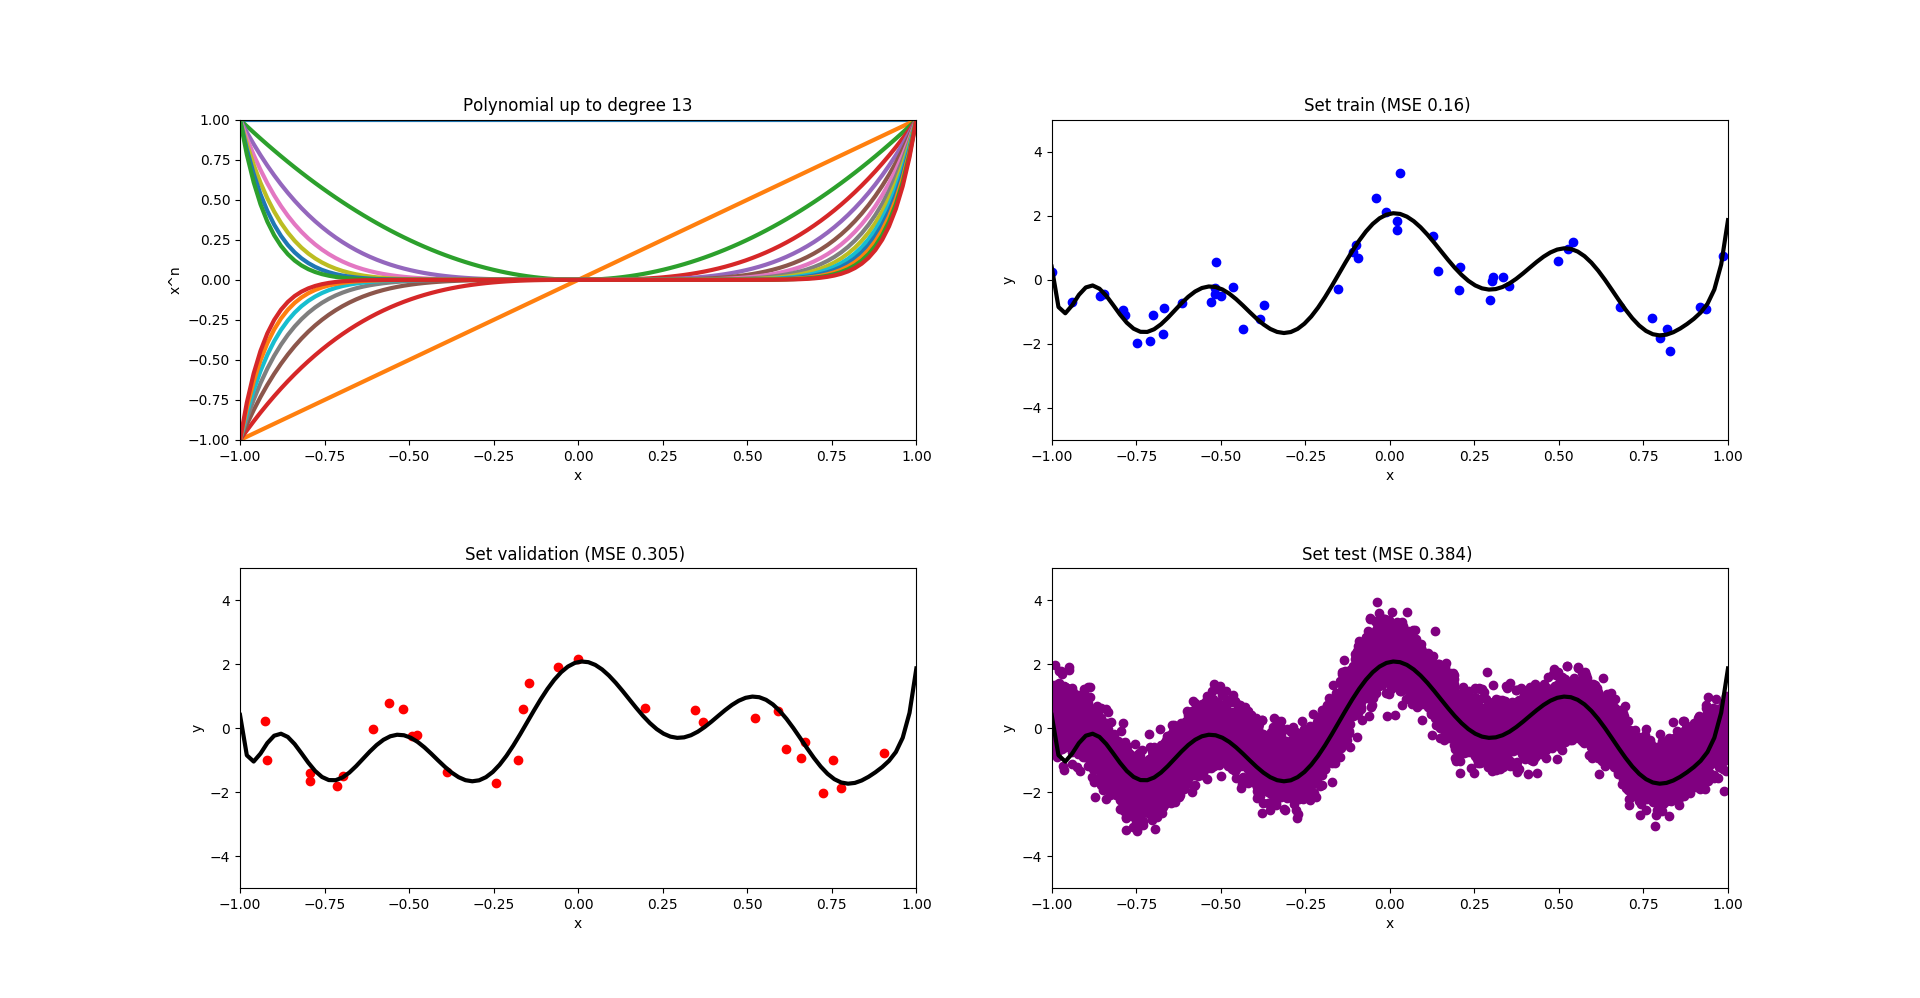
\includegraphics[width=\textwidth]{figures/linreg_degree_13.png}
	    \caption{Linear Regression (Polynomial, Degree 13)}
	\end{figure}
		
  \item \textbf{Discussion}\\
  Validation sets help to estimate performance of algorithms used for
  predictions and also to select a hypothesis (lowes error on set data).
  According to the error in the test set no over-fitting occured up to a
  degree of 13 (but would on higher degrees as can clearly be seen in Figure for
  degree 21, outliers and lesser data).
  
\end{itemize}
\subsection{Linear Regression with radial basis functions}
\begin{figure}[H]
	\centering
	        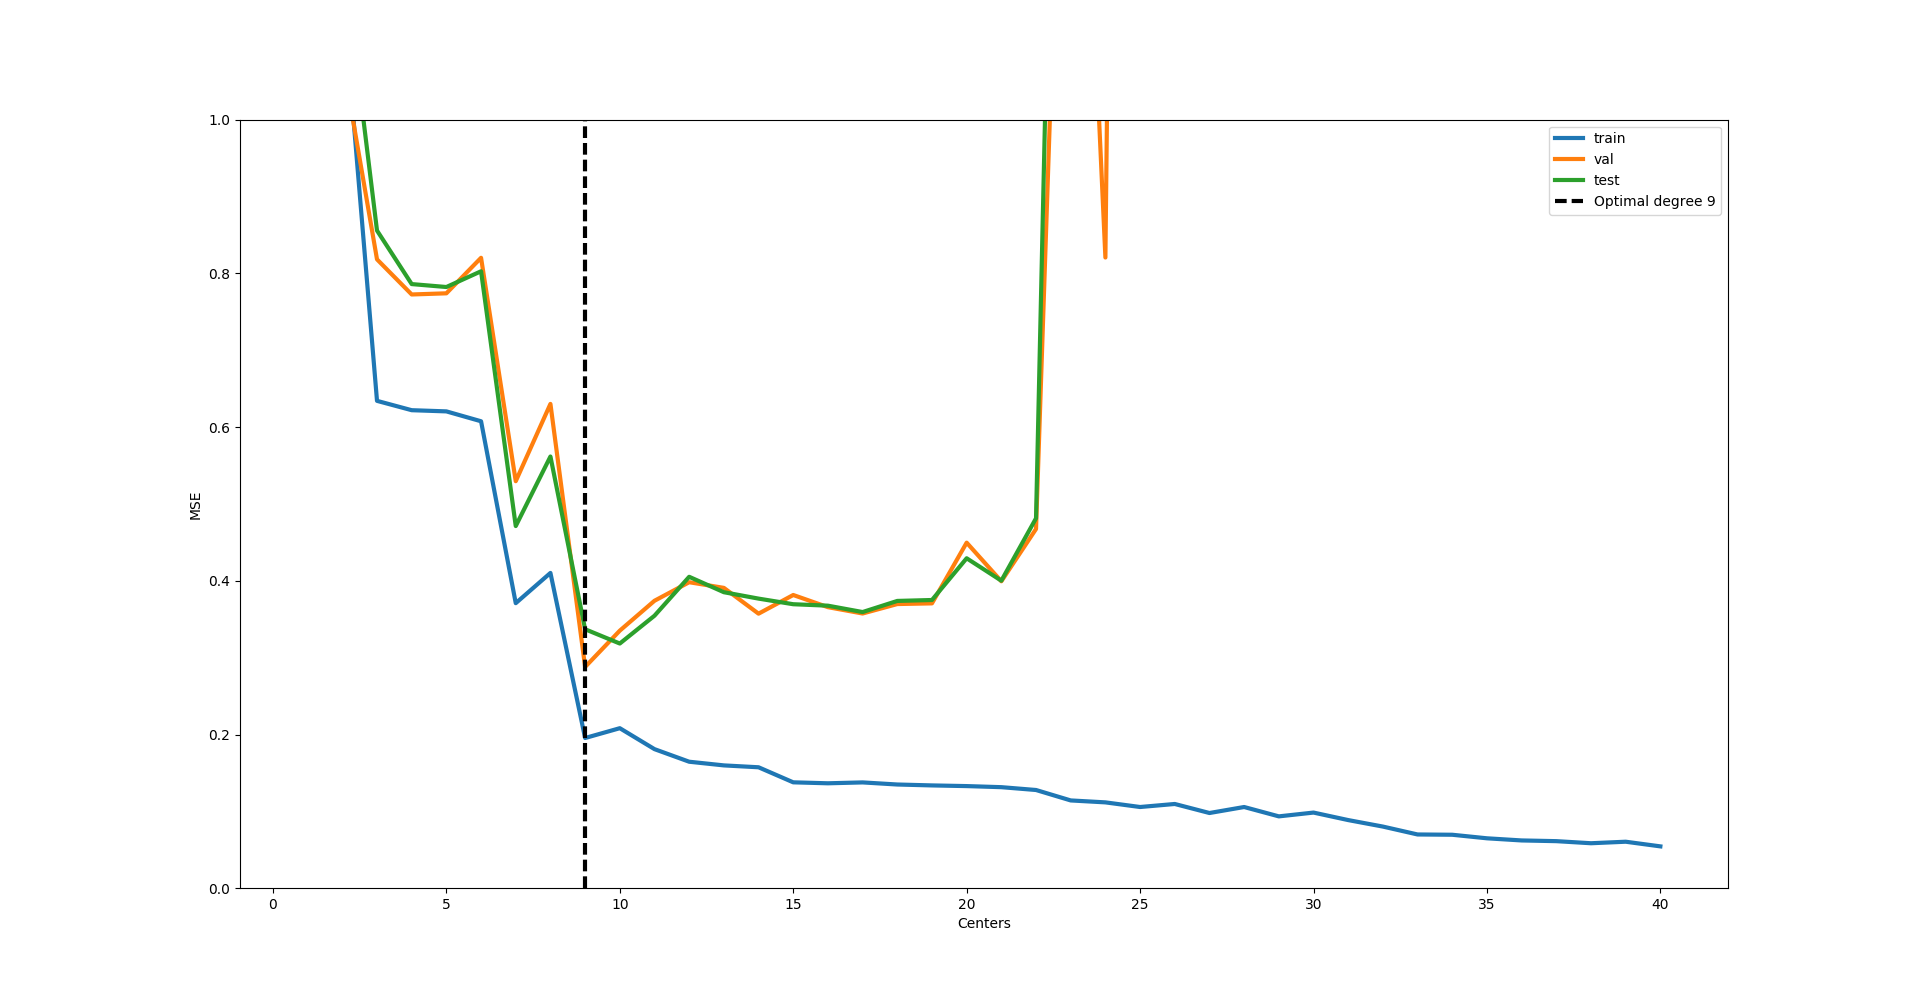
\includegraphics[width=\textwidth]{figures/linreg_bias_errors.png}
	    \caption{Training, validation and testing errors}
	\end{figure}
	\begin{figure}[H]
	\centering
	        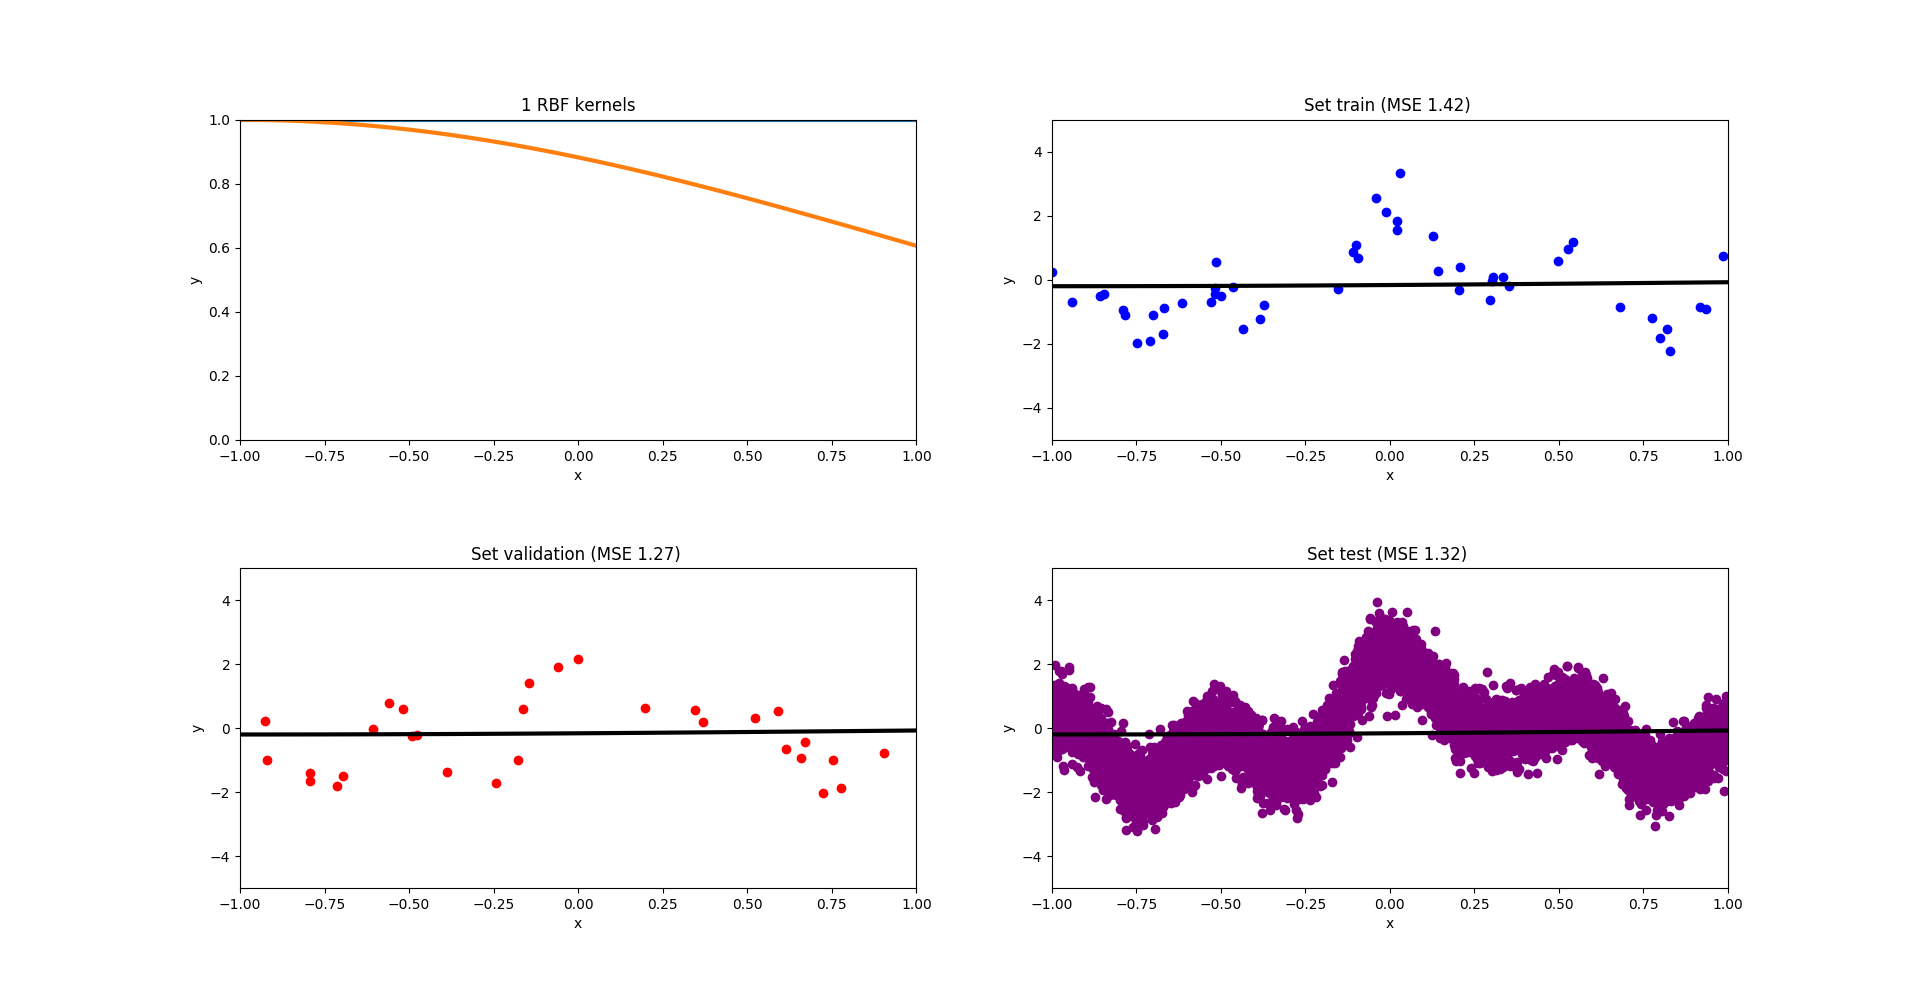
\includegraphics[width=\textwidth]{figures/linreg_bias_c1.png}
	    \caption{Linear Regression (Bias, Center 1)}
	\end{figure}
	\begin{figure}[H]
	\centering
	        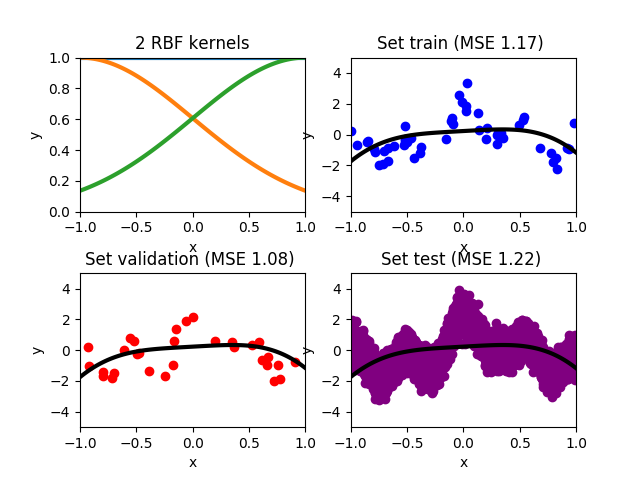
\includegraphics[width=\textwidth]{figures/linreg_bias_c2.png}
	    \caption{Linear Regression (Bias, Center 2)}
	\end{figure}
	\begin{figure}[H]
	\centering
	        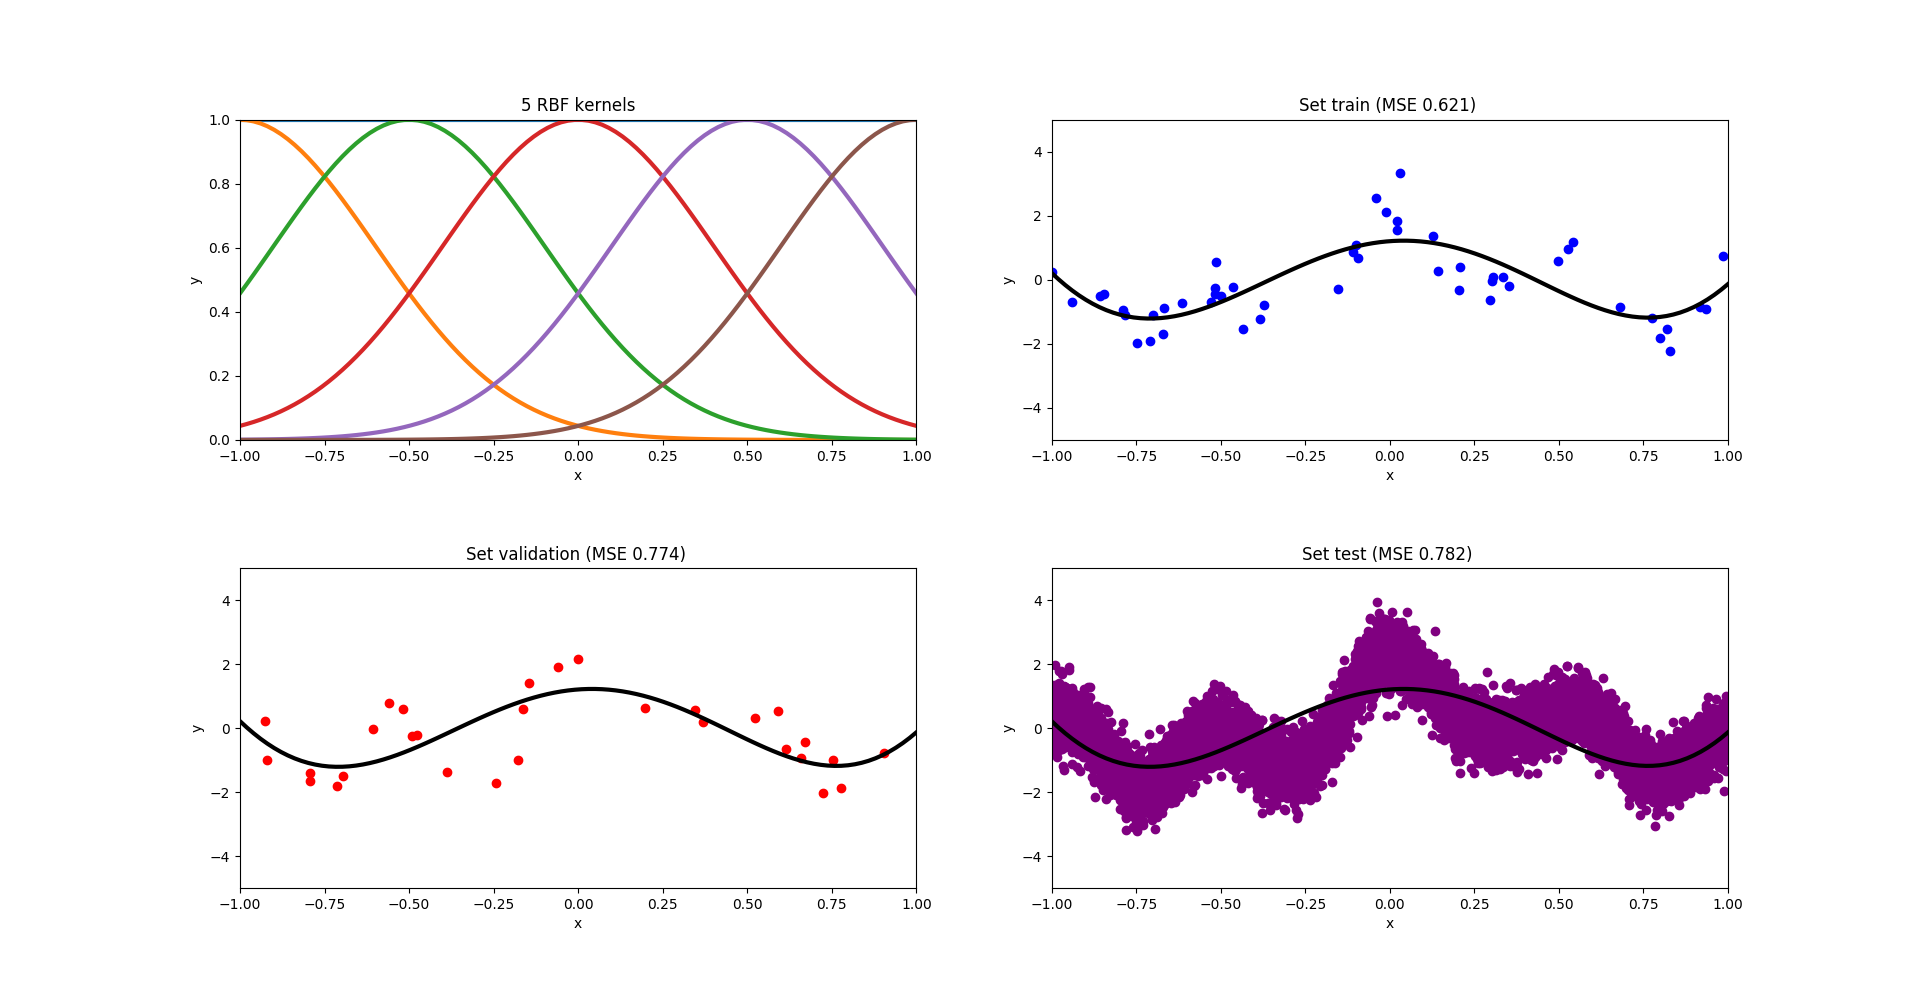
\includegraphics[width=\textwidth]{figures/linreg_bias_c5.png}
	    \caption{Linear Regression (Bias, Center 5)}
	\end{figure}
	\begin{figure}[H]
	\centering
	        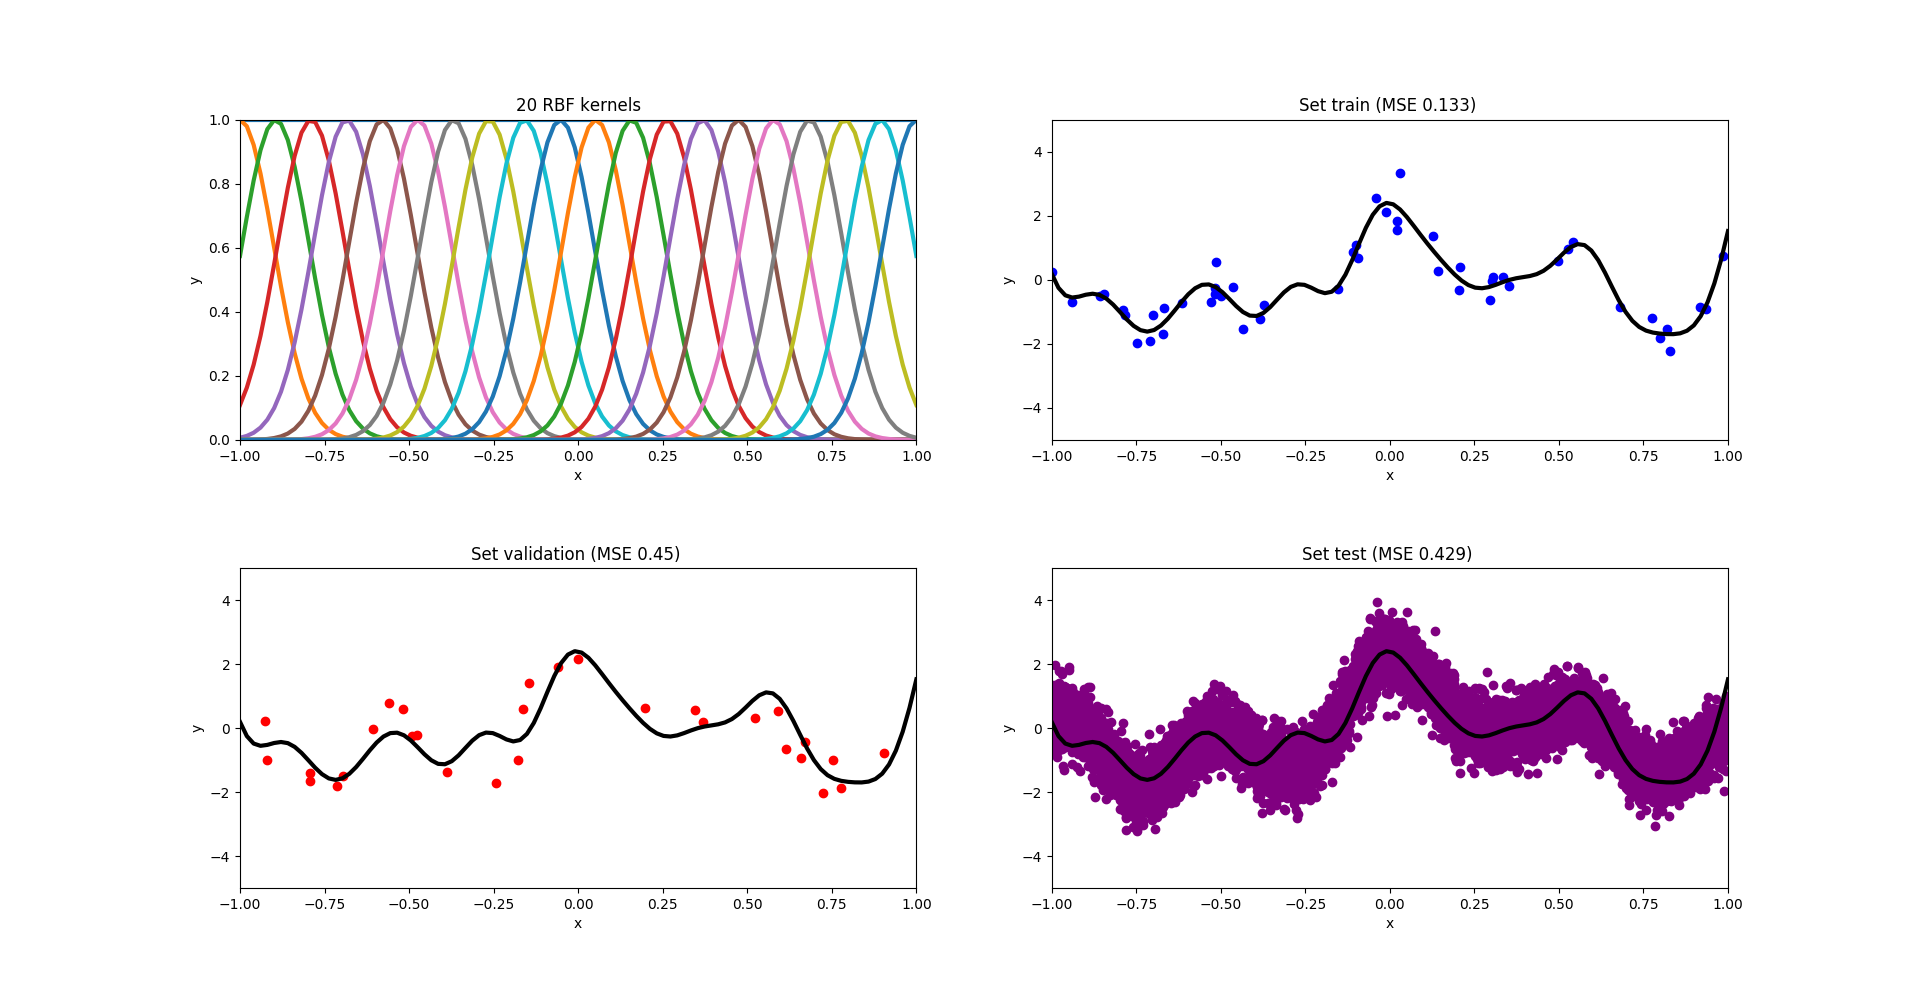
\includegraphics[width=\textwidth]{figures/linreg_bias_c20.png}
	    \caption{Linear Regression (Bias, Center 20)}
	\end{figure}
\begin{itemize}
  \item Lowest training error when using center 40
  	\begin{figure}[H]
    \centering
	        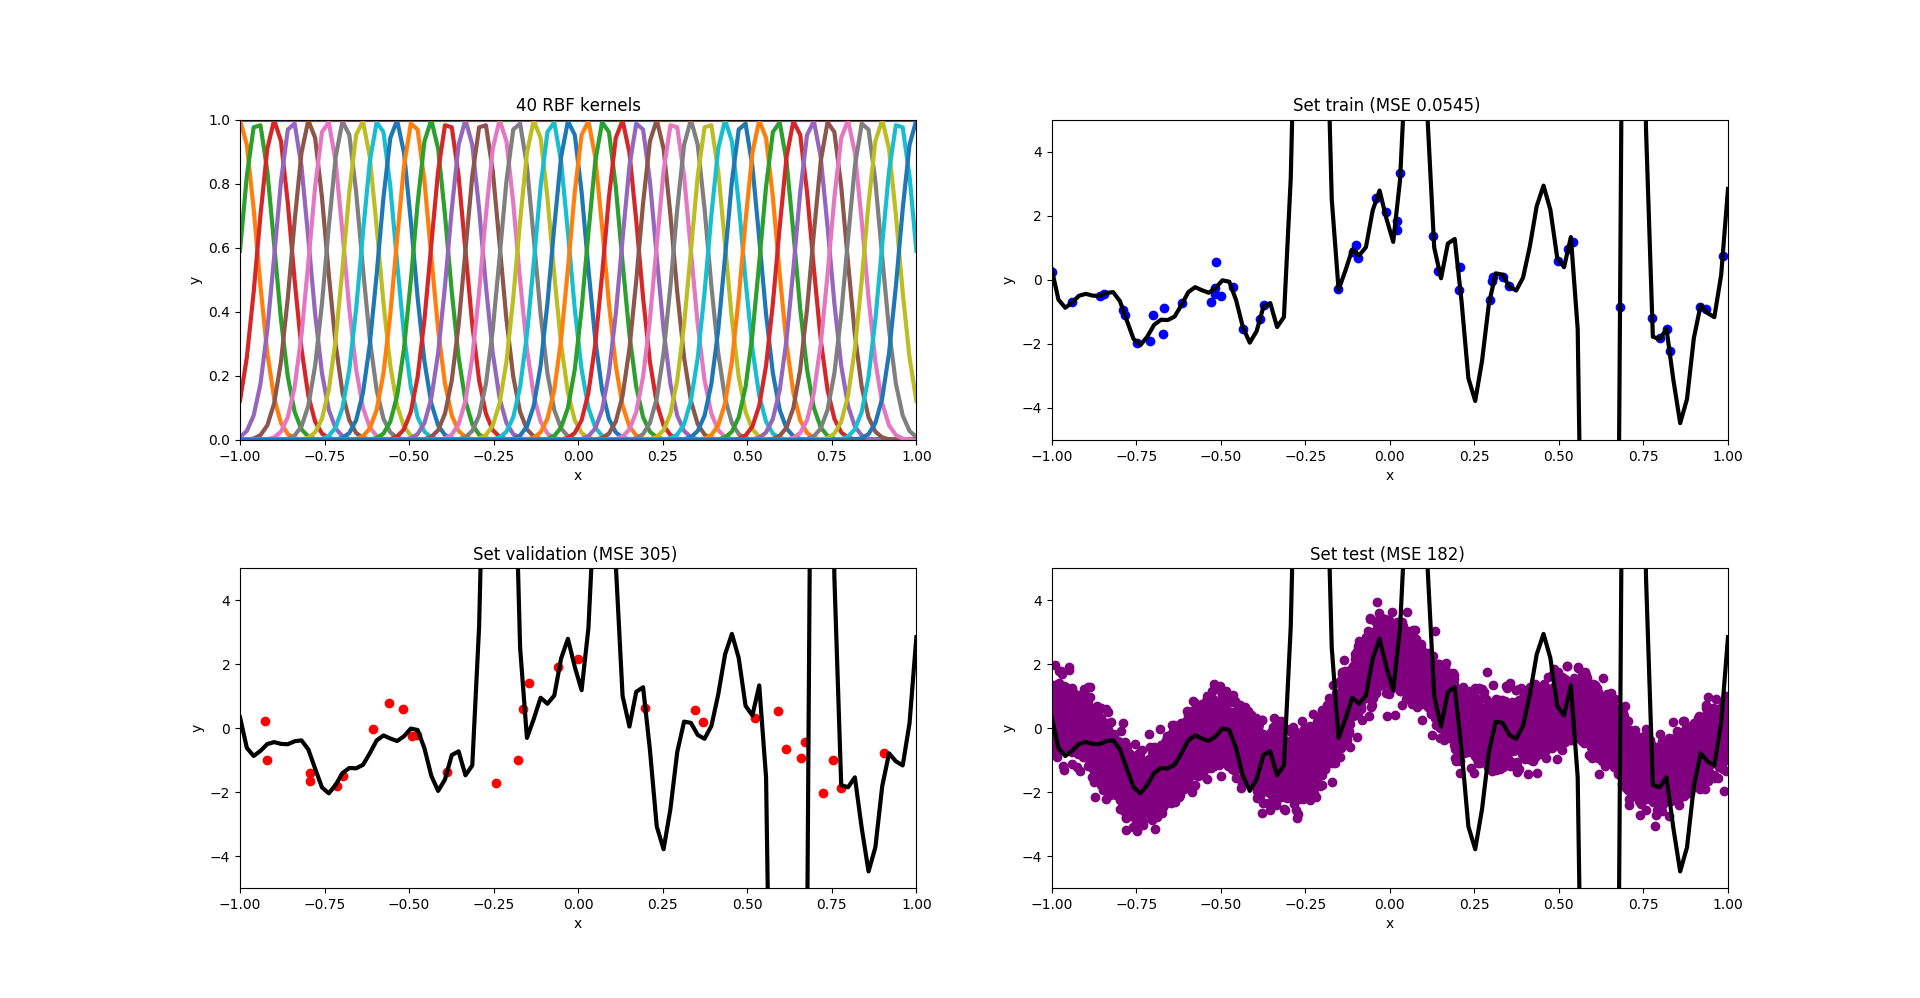
\includegraphics[width=\textwidth]{figures/linreg_bias_c40.png}
	    \caption{Linear Regression (Bias, Center 40)}
	\end{figure}
  \item Lowest validation error occurs when using center 9
	\begin{figure}[H]
    \centering
	        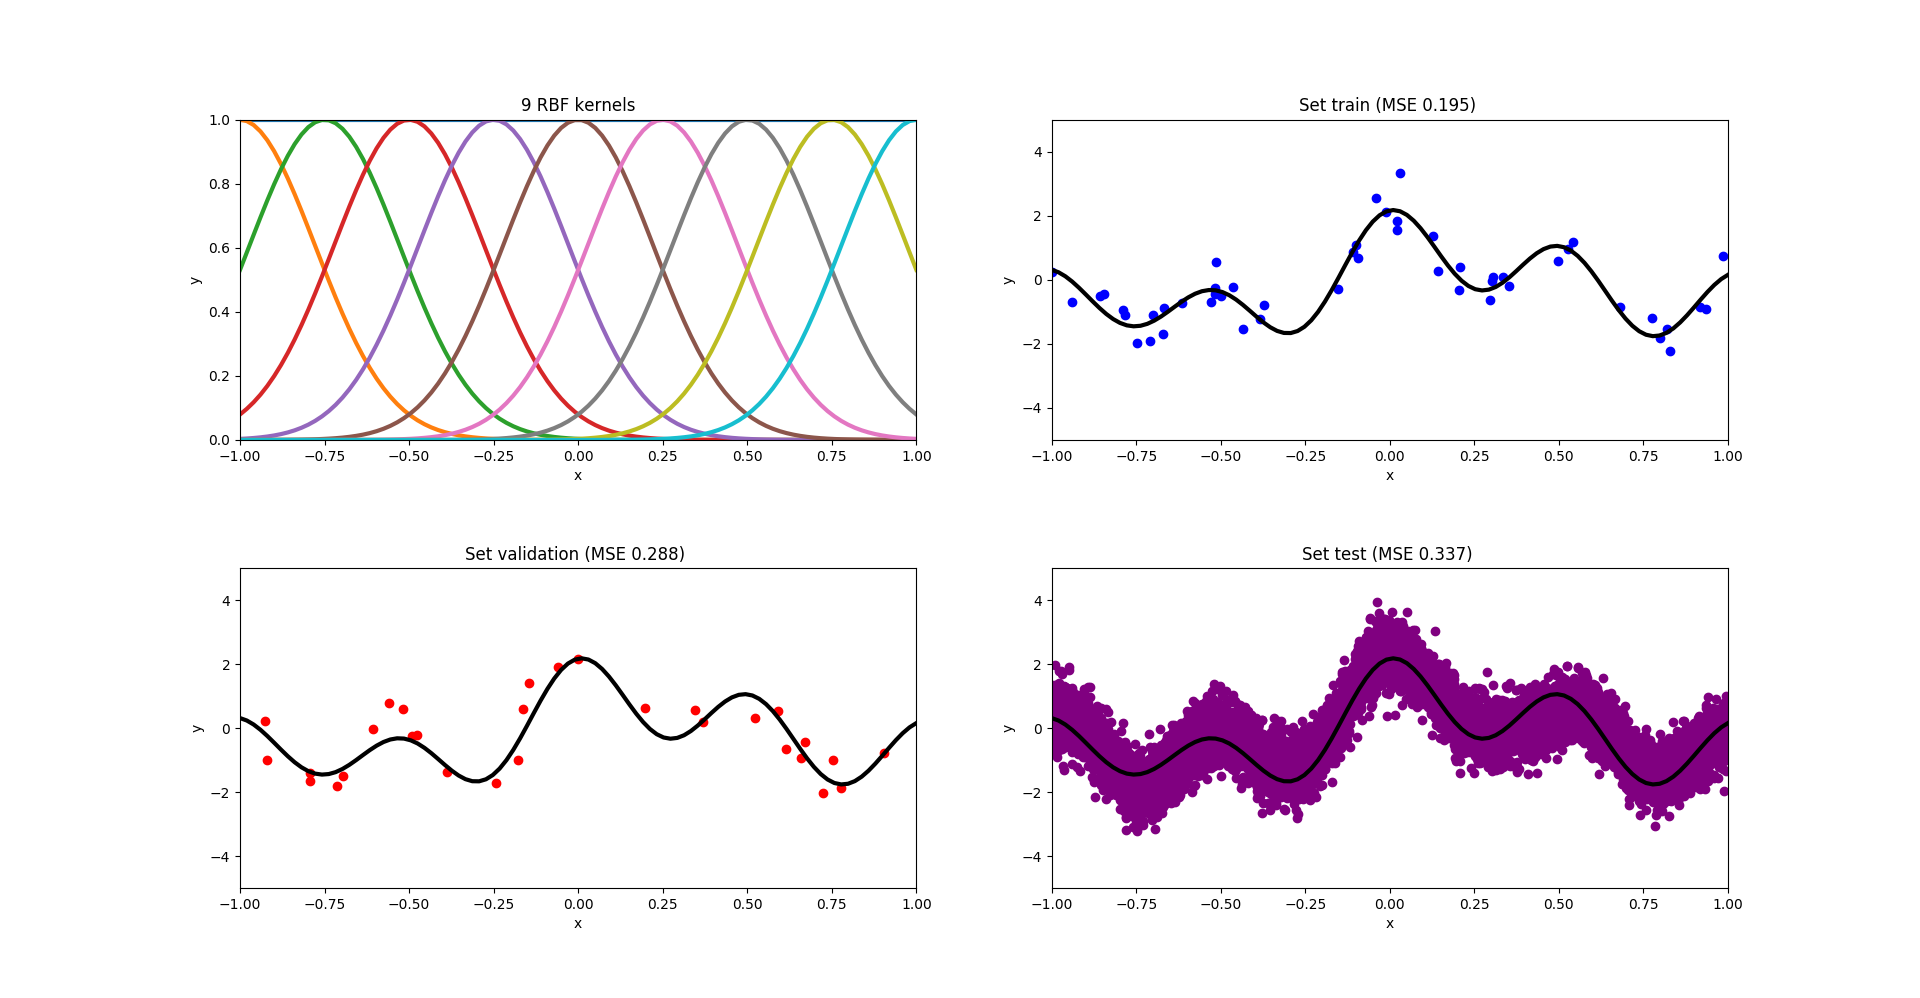
\includegraphics[width=\textwidth]{figures/linreg_bias_c9.png}
	    \caption{Linear Regression (Polynomial, Degree 9)}
	\end{figure}
		
  \item \textbf{Discussion}\\
  Bias function is better because it fits natural phenomen better. Overfitting
  occurs very early on parameter center 10.
  
\end{itemize}

\section{Logistic Regression}

\subsection{Derivation of Gradient}

\subsection{Logistic Regression training with gradient descent and scipy.optimize}

\subsubsection{Gradient descent}

\subsubsection{Adaptative gradient descent}

\subsubsection{Scipy optimizer}

\end{document}